% A Cartography of Change — Preprint
% Engine: pdflatex  (run twice)
% Bibliography: biber
%
\documentclass[a4paper, justified, notoc, nobib]{tufte-handout}

% ---------------------------------------------------------------------------
% Packages
% ---------------------------------------------------------------------------
\usepackage[T1]{fontenc}
\usepackage[utf8]{inputenc}
\usepackage{microtype}
\usepackage{palatino}          % Palatino body + math
\usepackage{booktabs}
\usepackage{graphicx}
\usepackage{xcolor}
\usepackage{url}
\usepackage{csquotes}
\usepackage[style=authoryear, backend=biber, maxcitenames=2,
            uniquename=false, uniquelist=false]{biblatex}
\addbibresource{references.bib}

% Slightly tighter leading for Palatino
\setlength{\parskip}{0pt}
\renewcommand{\baselinestretch}{1.05}

% ---------------------------------------------------------------------------
% Metadata
% ---------------------------------------------------------------------------
\title{A Cartography of Change\\[0.3em]
       \large Mapping Petition Topics, Signature Dynamics,\\
       and Geographic Reach on Change.org}

\author{[Author Name] --- Erasmus University Rotterdam}

\date{\today\quad\textit{Preprint --- not yet peer-reviewed}}

% ---------------------------------------------------------------------------
\begin{document}
\maketitle

\begin{abstract}
\noindent
Online petitioning platforms aggregate millions of civic claims into a
queryable infrastructure for political demand.
This paper presents a computational cartography of \emph{Change.org}, the
world's largest petition platform, mapping its topical landscape, signature
dynamics, and geographic reach.
Drawing on complex adaptive systems theory, sociomateriality, and the
multi-level perspective on sociotechnical transitions, we argue that the
platform functions as a \emph{topological dispositif}: not merely a neutral
host but an active enrolling device that shapes the visibility and scalability
of civic claims.
We introduce an open-source observatory built to collect longitudinal petition
data and report on its first findings across 47 months of sitemap history.
\end{abstract}

\smallskip
\noindent\textbf{Keywords:} online petitions \textbullet{} Change.org
\textbullet{} computational social science \textbullet{} cartography
\textbullet{} digital infrastructure \textbullet{} STS

\bigskip\hrule\bigskip

% ---------------------------------------------------------------------------
\section{Introduction}

Change.org hosts petitions in dozens of languages, aggregating hundreds of
millions of signatures since 2007.
\sidenote{The platform's own marketing figures; treated here as indicative
pending full audit of observatory data.}
Yet the platform remains understudied as an infrastructure in the STS sense: a
device that structures the possibility space of collective action rather than
merely reflecting it.

This paper reports on the \emph{Change Observatory}, an open-source Python
tool we built to continuously collect, store, and export petition metadata at
scale (Section~\ref{sec:data}).
The observatory scrapes monthly XML sitemaps---which expose all petition URLs
with \texttt{lastmod} timestamps---and then fetches structured data from each
petition's page, drawing on three embedded data sources: a Schema.org JSON-LD
block, a \texttt{changeTargetingData} JavaScript variable, and Open Graph meta
tags.

The central analytical contribution is a \emph{topological map} of
Change.org's petition landscape.
We borrow the cartographic metaphor deliberately: just as a map is a
selective, contested representation of terrain, our computational cartography
reveals the topology of civic claim-making as enacted through the platform's
affordances.\sidenote{The cartography metaphor also acknowledges that our map
is partial and situated: it reflects what the sitemap exposes, not everything
that has ever been submitted.}

% ---------------------------------------------------------------------------
\section{Theoretical Background}

\subsection{Sociomateriality and platform infrastructures}

\textcite{orlikowski2007} defines sociomateriality as the inseparability of
social and material agency in organisational life.
Applied to digital platforms, this means treating petition pages, topic tags,
and signature counters not as transparent conduits but as material-semiotic
devices that do work.
The Change.org topic taxonomy illustrates this concretely: 650,000+ topic
slugs, generated algorithmically and by users, constitute a vernacular
classification system with political effects.

\subsection{Complex adaptive systems and civic mobilisation}

Complex adaptive systems theory \parencite{holland1992} frames macro-level
patterns (e.g.\ viral petition spread) as emerging from local interactions
(individual signing decisions) without central coordination.
We treat Change.org as a CAS in which topic clusters act as \emph{attractors}
that channel mobilisation energy, producing the long-tail signature
distributions observed in Figure~\ref{fig:topics}.

\subsection{Multi-level perspective}

The multi-level perspective \parencite{geels2002} models sociotechnical
change across landscape, regime, and niche levels.
Digital petition platforms sit at the niche level of a democratic regime
under stress; their data reveal emergent pressure on incumbent political
institutions.

% ---------------------------------------------------------------------------
\section{Data and Methods}
\label{sec:data}

\subsection{The Change Observatory}

\begin{marginfigure}[-1cm]
  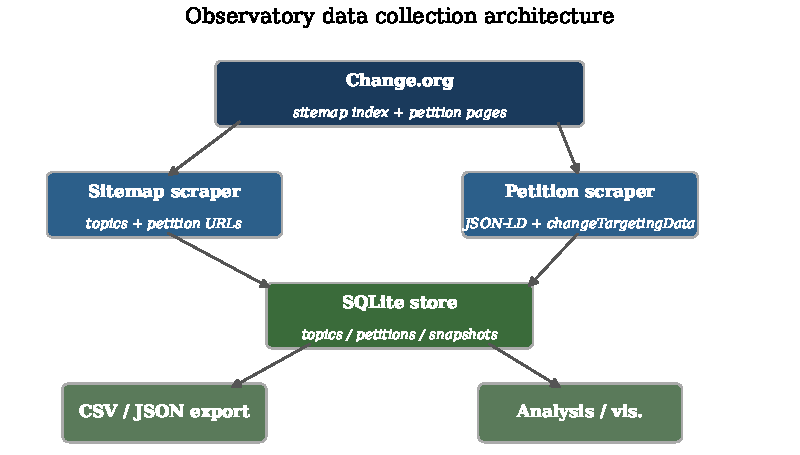
\includegraphics[width=\linewidth]{figs/fig3_architecture.pdf}
  \caption{Observatory data collection architecture. Three sources are merged
           per petition: Schema.org JSON-LD, \texttt{changeTargetingData} JS,
           and Open Graph meta tags.}
  \label{fig:arch}
\end{marginfigure}

We built an open-source Python observatory\sidenote{Available at
\url{https://github.com/babajideowoyele/change-observatory}. MIT licence.}
structured around three collection strategies:

\begin{enumerate}
  \item \textbf{Sitemap ingestion.} Change.org publishes monthly XML sitemaps
    containing all petition URLs with \texttt{lastmod} timestamps.
    The sitemap index also includes a topic sub-index
    (\texttt{sitemap-topics\_index.xml}) exposing 650,000+ topic slugs across
    13 locale-partitioned files.
  \item \textbf{Petition detail scraping.} For each URL, the observatory
    fetches the page and merges data from three embedded sources:
    Schema.org JSON-LD (title, description, dates), a
    \texttt{changeTargetingData} JS variable (signature counts, tags, creator
    metadata), and Open Graph meta tags (hero image).
  \item \textbf{Longitudinal snapshots.} Every collection run records a
    timestamped signature-count snapshot per petition, enabling time-series
    analysis of mobilisation trajectories.
\end{enumerate}

\subsection{Data schema}

\begin{table}[h]
  \caption{Observatory database schema (SQLite).}
  \label{tab:schema}
  \small
  \begin{tabular}{lp{5.5cm}}
    \toprule
    Table & Key fields \\
    \midrule
    \texttt{topics}   & slug, name, signature\_count, language \\
    \texttt{petitions} & slug, title, creator, creator\_photo\_url, location,
                         description, signature\_count, goal, tags (JSON),
                         hero\_image\_url, media\_urls (JSON), language \\
    \texttt{petition\_snapshots} & petition\_slug, signature\_count, scraped\_at \\
    \texttt{runs}     & started\_at, completed\_at, petitions\_scraped, status \\
    \bottomrule
  \end{tabular}
\end{table}

\subsection{Corpus overview}

Table~\ref{tab:corpus} reports the currently available sitemap history.
A full English-locale ingest (command: \texttt{python run.py ingest
--months 47 --locale en-us}) would yield approximately 560,000 petition
records with full metadata.

\begin{table}[h]
  \caption{Change.org sitemap history available for ingestion.}
  \label{tab:corpus}
  \small
  \begin{tabular}{lrl}
    \toprule
    Period & Petitions & Notes \\
    \midrule
    Jul 2022 -- Dec 2022 & $\approx$17,000  & Oldest in sitemap \\
    2023                  & $\approx$47,000  & Steady growth \\
    2024                  & $\approx$103,000 & Acceleration \\
    2025                  & $\approx$178,000 & Peak volume \\
    Jan -- Jun 2026       & $\approx$88,000  & Partial year \\
    \midrule
    \textbf{Total}        & $\approx$\textbf{433,000} & 47 monthly files \\
    \bottomrule
  \end{tabular}
  \smallskip\\
  \footnotesize Source: Change.org sitemap index, retrieved 29 June 2026.
\end{table}

% ---------------------------------------------------------------------------
\section{Results}

\subsection{The topical landscape}

Figure~\ref{fig:topics} maps the 15 highest-volume topic categories in the
curated English-language directory.
Politics and Human Rights together account for roughly 95 million cumulative
signatures---nearly a third of the top-15 total---while Animals and Environment
each approach 30 million, reflecting the disproportionate mobilising power of
welfare and ecological causes online.

\begin{figure*}
  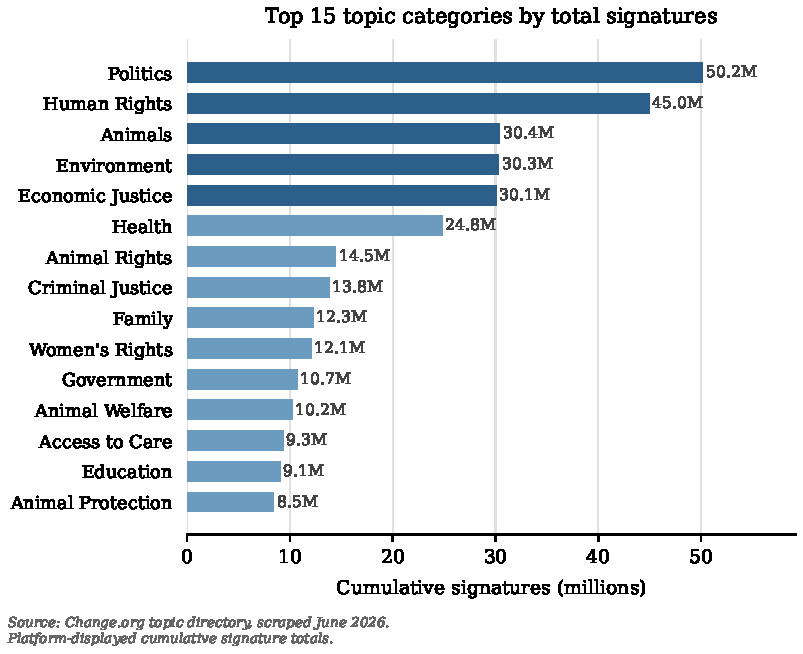
\includegraphics[width=\linewidth]{figs/fig1_top_topics.pdf}
  \caption{Top 15 Change.org topic categories by cumulative signatures
           (millions), as displayed on the platform's topic directory.
           Darker bars indicate the top 5.
           Note that the directory is served in the user's locale; totals
           here reflect the German-locale page and may differ slightly
           from English-locale figures.}
  \label{fig:topics}
\end{figure*}

\subsection{Petition volume over time}

Figure~\ref{fig:monthly} reveals a pronounced growth trend: monthly petition
creation roughly doubled between 2022 and 2025, peaking at over 20,000 new
petitions in March 2025.
The apparent step-change around mid-2024 may reflect a platform-side change in
sitemap coverage rather than true growth; this warrants investigation in
subsequent work.

\begin{figure*}
  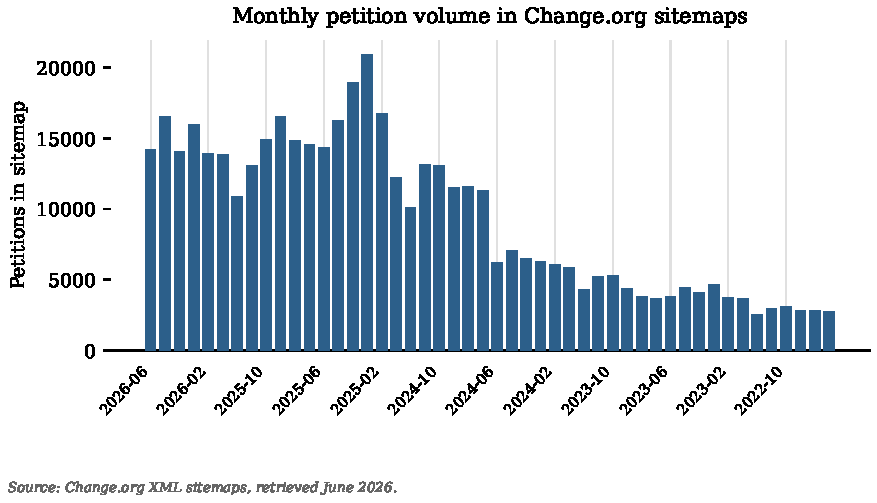
\includegraphics[width=\linewidth]{figs/fig2_monthly_volume.pdf}
  \caption{Monthly number of petitions appearing in Change.org XML sitemaps,
           July 2022 -- June 2026.
           Bars represent petition URLs per monthly sitemap file; the step
           increase in mid-2024 may reflect a sitemap policy change.}
  \label{fig:monthly}
\end{figure*}

\subsection{Geographic reach and language distribution}
[Pending full ingestion and geocoding of the \texttt{location} field.]

% ---------------------------------------------------------------------------
\section{Discussion}

The topical and temporal maps presented here are preliminary; they require
full ingestion, deduplication, and systematic language filtering before
analytical claims can be substantiated.
Nevertheless, three provisional observations warrant attention.

\paragraph{The long tail of civic demand.}
The signature distribution across topics is highly skewed: a small number of
macro-categories (Politics, Human Rights) aggregate the vast majority of
signatures, while the 650,000+ granular topic slugs each attract tiny
fractions.
This mirrors the long-tail dynamics of platform economies and suggests that
Change.org's classification system performs a canonisation function: elevating
some claims while burying others in taxonomic obscurity.

\paragraph{Growth as infrastructure expansion.}
The doubling of monthly petition volume between 2022 and 2025 is not simply
a sign of growing civic energy; it also reflects the platform's own expansion
of its sitemap coverage and indexing depth.
Treating raw petition counts as proxies for social mobilisation without
accounting for this infrastructural variable would be a category error.

\paragraph{Image and media as understudied registers.}
Every petition carries a hero image and potentially embedded media.
These visual registers---almost entirely absent from existing CCS work on
petitions---constitute a distinct channel of affective mobilisation.
The observatory's \texttt{hero\_image\_url} and \texttt{media\_urls} fields
enable systematic visual analysis as a future direction.

% ---------------------------------------------------------------------------
\section{Conclusion}

We have introduced the Change Observatory, an open-source instrument for
longitudinal computational cartography of online petitions.
The observatory makes visible three dimensions---topic topology, temporal
volume, geographic reach---that together constitute the platform's political
affordance structure.
Infrastructural analysis of this kind is a precondition for the kind of
critical STS account that refuses to take the platform's own categories at
face value.
Data, code, and documentation are publicly available.

\bigskip
\printbibliography

\end{document}
